\documentclass[14pt]{extarticle}
\usepackage[utf8]{inputenc}
\usepackage{ngerman}
\usepackage{array}
\usepackage{amsmath}
\usepackage{graphicx}
\title{Bericht Todesstern U3}
\author{Charline Waldrich, Robert Ullmann, Julian Dobrot}
\date{13. november 2015}

\begin{document}

\maketitle
\pagebreak
\tableofcontents


\section{Aufgabenstellung}
Implementierung von Beleuchtung im todesstern Raytracer.
\subsection{Änderungen an bestehenden Klassen}
\subsubsection{Änderungen am Hit-Objekt}
\subsubsection{Änderungen an der Geometrie-Klasse und am Dreieck}
\subsubsection{Änderungen an der World-Klasse}
\subsubsection{Demo-Szene}

\subsection{Licht}
\subsubsection{Light}
\subsubsection{PointLight}
\subsubsection{DirectionalLight}
\subsubsection{SpotLight}

\subsection{Material}
\subsubsection{SingleColorMaterial}
\subsubsection{LambertMaterial}
\subsubsection{PhongMaterial}


\section{Lösungsstrategien}
Allgemein wurden als erster Lösungsschritt alle aus der Aufgabenstllung hervorgehenden Klassendiagramme komplett in das Projekt integriert.


\section{Implementierungen}




\section{Besondere Probleme oder Schwierigkeiten bei der Bearbeitung}



\section{Zeitbedarf}
\begin{center}
\begin{tabular}{cr}
Strahl	  \	&60 min	\\
Kameras 	\	&120 min	\\
Farben \	&60 min	\\
Geometrien \	&720 min	\\
Welt \	&60 min	\\
Raytracer \	&240 min	\\
Bericht  \		&180 min	 \\
	\hline
	&1440 min
\end{tabular}
\end{center}

\subsection{Tests}
\subsubsection{Abbildung 3}
Demo Szene mit einfarbigen Material.\\
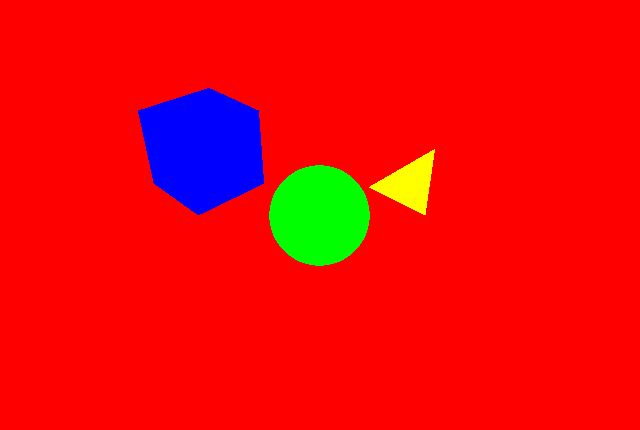
\includegraphics[width=15cm,height=10cm]{images/Abbildung3}\\



\section{Quellen}

\end{document}
